\section*{Problem 2: findRange} 


\textbf{a)} Betrachten Sie den folgenden binären Suchbaum:
\noindent
Wo befinden sich die Schlüssel, die kleiner sind als 37? Wo befinden sich die
Schlüssel, die größer sind als 21? Wo befinden sich die Schlüssel, die zwischen
21 und 37 liegen?

\begin{center}
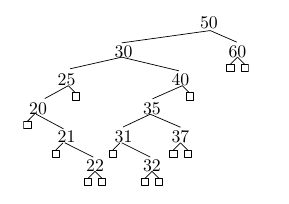
\includegraphics[scale=1]{Aufgabe2}
\end{center}

\noindent
\textbf{b)} Beschreiben Sie, wie man in einem AVL-Baum mit $n$ Schlüsseln die Operation
findRange(k1 , k2 ) implementieren kann, die alle Schlüssel $k$ liefert, für die
$k1 \leq k \leq k2$ ist. Die Laufzeit soll $O(log n + s)$ betragen. Dabei ist s die Anzahl
der gelieferten Schlüssel.




 







